\documentclass[a4paper]{article}
\usepackage[utf8]{inputenc}
\usepackage[russian,english]{babel}
\usepackage[T2A]{fontenc}
\usepackage[left=10mm, top=20mm, right=18mm, bottom=15mm, footskip=10mm]{geometry}
\usepackage{indentfirst}
\usepackage{amsmath,amssymb}
\usepackage[italicdiff]{physics}
\usepackage{graphicx}
\usepackage{siunitx}
\graphicspath{{images/}}
\DeclareGraphicsExtensions{.pdf,.png,.jpg}
\usepackage{wrapfig}

\usepackage{caption}
\captionsetup[figure]{name=Рисунок}
\captionsetup[table]{name=Таблица}

\title{\underline{Вопрос по выбору (Термодинамика)}}
\author{Воронин Денис, Б04-407}
\date{}
\begin{document}

\maketitle
\begin{center}
\textbf{\Large Квантовая теория теплоемкости (Эйнштейна)}
\end{center}

\section{Введение}

В соответствии с законами классической механики на каждую степень свободы молекулы
(точнее — на каждое квадратичное по координате или скорости слагаемое в энергии) приходится теплоемкость
$\frac{R}{2}$ (в расчете на моль вещества). В частности, для газа, состоящего из двухатомных молекул, теплоемкость
складывается из поступательной, вращательной и колебательной частей и равна
\[C_{V} = E_{\text{пост.}}+E_{\text{вращ.}}+E_{\text{колеб.}}= \frac{3R}{2}+\frac{2R}{2}+(\frac{R}{2}+\frac{R}{2})=\frac{7R}{2}\]

Эта формула говорит о том, что теплоемкость должна быть постоянной и не зависеть от температуры. 
Но опыты показывают, что она от нее зависит. Ниже приведен график зависимости теплоемкости от температуры (рис.1). Далее будет приведен график, который наглядно покажет зависимость теплоемкости 
некоторых веществ от температуры:

\begin{figure}[htbp]
    \centering
    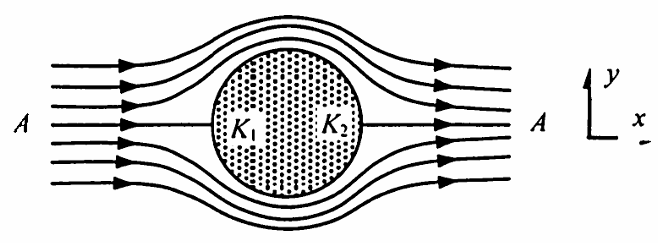
\includegraphics[width=0.45\textwidth]{pick1.png}
    \caption{Зависимость теплоемкости от температуры(для двухатомной молекулы)}
    \label{fig:example}
\end{figure}

При высоких температурах работает теорема о равнораспределении энергии по степеням свободы. 
При низких температурах замораживаются сначала колебательные, а затем вращательные степени свободы. Тогда при достаточно
низких температурах молекула ведет себя как система, обладающая только поступательными степенями свободы.
Оказалось, что колебательные степени замерзают при $T\sim 1000 K - 10000 K$, а вращательные при $T\sim 100 K$.\par
Далее для рассмотрения этого вопроса обратимся к кватовой теории, а именно рассмотрим предложенную Эйнштейном модель, иллюстрирующую «включение» колебательных степеней 
свободы по мере роста температуры.

\section{Вывод формулы теплоемкости кристалла}

Двухатомную молекулу при не слишком высоких энергиях можно рассматривать как одномерный гармонический осциллятор.
Из законов квантовой механики энергия гармонического осциллятора с классической частотой $\omega $ может принимать только дискретный набор значений
 
\[\varepsilon_{n} = (n+\frac{1}{2})\hbar \omega\]
где n= 0,1,2,3\dots \par
Далее из распределения Гиббса, вероятность того, что молекула обладает энергией $\varepsilon_{n}$ равна
\[W_{n}=\frac{1}{Z}\exp(-\frac{\varepsilon_{n}}{KT})\]

Найдем статистическую сумму Z. Введем обозначение $\beta =\frac{1}{KT}$ получаем:
\[Z= \sum_{n = 0}^{\infty} \exp(-\beta \varepsilon_{n})=\exp(-\frac{1}{2} \beta \hbar \omega)\sum_{n = 0}^{\infty} \exp(-n\beta \hbar\omega)\underbrace{=}_{\text{геом. прогр.}} \frac{\exp(-\beta \hbar \omega/2)}{1-\exp(-\beta \hbar \omega)}\]

Зная Z, можно найти среднюю энергию молекулы, но перед этим покажем связь производной и энергии:

\begin{align*}
\frac{\partial Z}{\partial \beta} = \sum_n \frac{\partial}{\partial \beta} [\exp(-\beta \varepsilon_n)] = \sum_n (-\varepsilon_n) \exp(-\beta \varepsilon_n)
\end{align*}

\begin{align*}
\frac{\partial \ln Z}{\partial \beta} \,=\, \frac{1}{Z}\,\frac{\partial Z}{\partial \beta}\,=\,\frac{1}{Z}\,\sum_n (-\varepsilon_n) \exp(-\beta \varepsilon_n)\,=\, -\sum_n \varepsilon_n \underbrace{\frac{\exp(-\beta \varepsilon_n)}{Z}}_{W_n}\,=\, - \bar{\epsilon}
\end{align*}

Откуда и получаем, что $\varepsilon =-\frac{\partial lnZ}{\partial \beta}$. Возвращаясь к энергии имеем:

\[\overline{\epsilon}= \sum_{n = 0}^{\infty} \varepsilon_{n}W_{n} = -\frac{\partial lnZ}{\partial \beta}=-\frac{\partial}{\partial \beta}(-\frac{1}{2}\beta \hbar \omega - ln(1-e^{-\beta \hbar \omega}))\underbrace{=}_{\text{(3)}} \frac{1}{2}\hbar \omega cth(\frac{\hbar \omega}{2KT})\]  

\rule{0.5\linewidth}{0.4pt}

\textbf{ Пояснение к (3) шагу}:

\[
\frac{\partial}{\partial \beta} \left[ - \ln(1 - \exp(-\beta \hbar \omega)) \right] = -\frac{1}{1 - \exp(-\beta \hbar \omega)} \cdot \frac{\partial}{\partial \beta} \left[ 1 - \exp(-\beta \hbar \omega) \right]
\]

\[
\frac{\partial}{\partial \beta} \left[ 1 - \exp(-\beta \hbar \omega) \right] = -[-\hbar \omega \exp(-\beta \hbar \omega)] = \hbar \omega \exp(-\beta \hbar \omega)
\]

Подставляем:

\[
- \frac{1}{1 - \exp(-\beta \hbar \omega)} \cdot \hbar \omega \exp(-\beta \hbar \omega) = -\hbar \omega \frac{\exp(-\beta \hbar \omega)}{1 - \exp(-\beta \hbar \omega)}
\]

Собираем обе части:

\[
\frac{\partial \ln Z}{\partial \beta} = -\frac{\hbar \omega}{2} - \hbar \omega \frac{\exp(-\beta \hbar \omega)}{1 - \exp(-\beta \hbar \omega)}
\]

Делаем последние преобразования:

\begin{align*}
\bar{\epsilon} = \frac{\hbar\omega}{2} + \frac{\hbar\omega}{\exp(\beta\hbar\omega) - 1} = \hbar\omega\left[\frac{1}{2} + \frac{1}{\exp(\beta\hbar\omega) - 1}\right]
\end{align*}

\begin{align*}
\bar{\epsilon}=\hbar\omega\left[\frac{\exp(\beta\hbar\omega)-1}{2(\exp(\beta\hbar\omega)-1)}+\frac{2}{2(\exp(\beta\hbar\omega)-1)}\right]=\hbar\omega\left[\frac{\exp(\beta\hbar\omega)-1+2}{2(\exp(\beta\hbar\omega)-1)}\right]
\end{align*}

\begin{align*}
\overline{\epsilon}=\hbar\omega\left[\frac{\exp(\beta\hbar\omega)+1}{2(\exp(\beta\hbar\omega)-1)}\right]=\frac{\hbar\omega}{2}\cdot\frac{\exp(\beta\hbar\omega)+1}{\exp(\beta\hbar\omega)-1}
\end{align*}

\rule{0.5\linewidth}{0.4pt}

Соответственно, энергия 1 моля рассмотриваеемых молекул составит $E = N_{A}\overline{\epsilon} $ и для молярной теплоемкости 
получем:
\[C_{V} = (\frac{\partial E}{\partial T})_{V} = R(\frac{\hbar \omega}{2kT})^{2}\frac{1}{sh^{2}(\hbar \omega/2kT)}\]
Получили выражение, определяющее теплоемкость системы молекул, имеющих одну колебательную степень свободы.\par
Т.к. в кристалле каждый атом может рассматриаться как 3-х мерный осциллятор, то утроив полученное выражение выше получим теплоемкость системы для кристалла.
\[C_{V} = 3R(\frac{\hbar \omega}{2kT})^{2}\frac{1}{sh^{2}(\hbar \omega/2kT)}\]

Формула для $C_{p}$ выглядит следующим образом:

\[C_{p} = C_{v}+ \frac{\alpha^{2}VT}{\beta_{T}}\]
\newpage
Где:

\begin{itemize}
    \item $\alpha$ — коэффициент теплового расширения,
    \item $V$ — объём,
    \item $\beta_T$ — изотермическая сжимаемость,
    \item $T$ — температура.
\end{itemize}

При низких температурах, как следует из найденной формулы,
теплоемкость убывает до нуля при $T\rightarrow 0$ по закону
\[C_{V} = 3R(\frac{\hbar \omega}{2kT})^{2}\exp(-\frac{\hbar \omega}{kT})\]

Физической причиной такого поведения теплоемкости является
дискретность энергетических уровней осциллятора (рис.2).
При высоких температурах, когда $kT \gg  \hbar \omega$ дискретность не проявляется, поскольку в диапазон значений энергии $\sim kT$ попадает много энергетических уровней осциллятора (рис.2а).
Поэтому система ведет себя как классическая. При низких же температурах
$kT\ll \omega$характерная тепловая энергия мала по сравнению с расстоянием между энергетическими уровнями (рис.2б). В результате
лишь малая доля молекул $\backsim \exp (-\hbar \omega/kT)$ оказывается вовлеченной
в колебательное движение. Большая же часть молекул остается в основном (невозбужденном) состоянии. Это и проявляется в убывании
теплоемкости по мере уменьшения температуры

\begin{figure}[htbp]
    \centering
    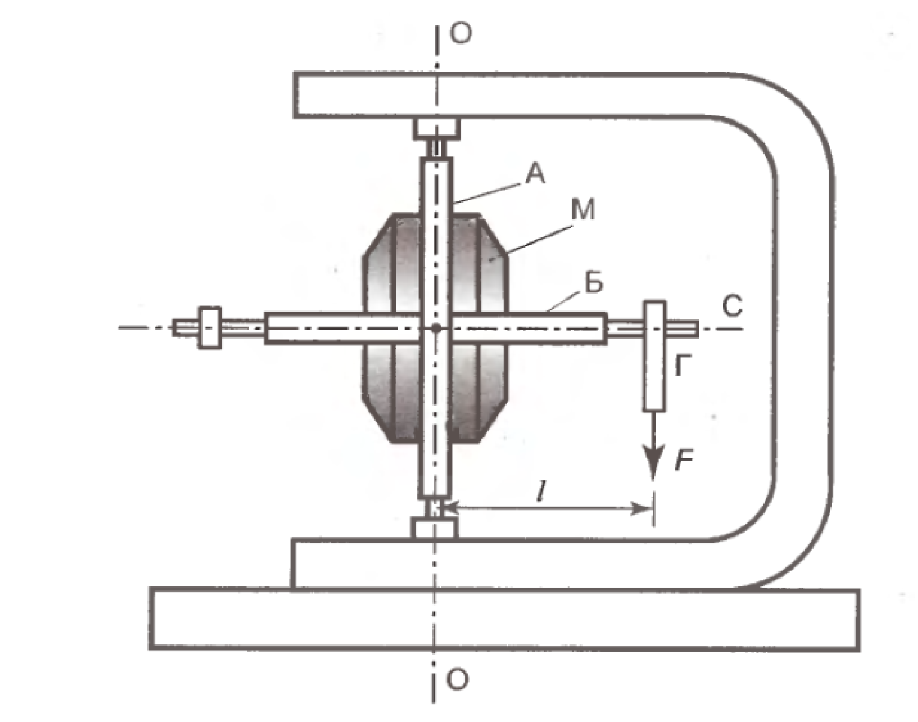
\includegraphics[width=0.45\textwidth]{pick2.png}
    \caption{Система уровней осцилятора и характерный масштаб энергий}
    \label{fig:example}
\end{figure}

\section{Условия применимости колебательной степени свободы}

Величину $T_{\text{колеб.}}= \frac{\hbar \omega}{k}$ называют характеристической температурой, определяющей условие возбуждения колебательных 
степеней свободы: при $T\gg T_{\text{колеб.}}$ колебательные степени активны, а при
$T\ll  T_{\text{колеб.}}$ эти степени свободы «заморожены».

\section{Вращательные степени свободы}

Помимо колебательных степеней свободы система может обладать
и вращательными степенями. Согласно квантовой механике ротатор
(линейная молекула) имеет серию вращательных уровней, энергия
которых дается формулой
\[\epsilon_{\text{вращ.}}= Bl(l+1), l=0,1,2 \dots\]

Величина l называется вращательным квантовым числом, а константа B называется вращательной постоянной и связана с моментом
инерции молекулы I соотношением
\[B = \frac{\hbar^{2}}{2I}\]

В соответствии со сказанным выше вращательные степени свободы молекулы возбуждаются, если температура достаточно 
велика: $T\gg T_{\text{вращ.}}$, где характеристическая температура для вращательного
движения определяется равенством $T_{\text{вращ.}} = \frac{B}{k}=\frac{\hbar^{2}}{2kI}$. В противоположном случае  $T\ll T_{\text{вращ.}}$ вращательные степени свободы остаются
«замороженными».

\section{Модель Дебая}

Центральным элементом модели Дебая является линейное дисперсионное соотношение $\omega = vq$, где $\omega$ — частота колебаний, $v$ — скорость звука в материале, а $q$ — волновое число. Это соотношение характеризует акустические моды колебаний, которые преобладают при низких энергиях и
малых значениях $q$. Линейность дисперсионного соотношения обеспечивает корректное описание теплоемкости при низких температурах, когда термически возбужденными остаются лишь низкоэнергетические фононы. Однако стоит отметить, что данное предположение становится менее точным для высокоэнергетических фононов, где нелинейные эффекты начинают играть заметную роль. Тем не менее, для большинства кристаллических материалов модель Дебая демонстрирует высокую степень согласия с экспериментальными данными в широком диапазоне температур.

Одним из наиболее значительных достижений модели Дебая является точное описание зависимости теплоемкости от температуры при низких температурах. В этом режиме теплоемкость пропорциональна кубу температуры (закон $T^3$), что выражается формулой
\[
C_V(T) = \frac{12}{5}\pi^4 N k_B \left(\frac{T}{T_D}\right)^3,
\]
где $N$ — число атомов в решетке, $k_B$ — постоянная Больцмана, $T_D$ — температура Дебая. Этот закон подтверждается экспериментально для многих кристаллических материалов, таких
как алмаз, где даже комнатная температура может считаться ``низкой'' в контексте модели из-за высокого значения $T_D$ (например, 2230 К для алмаза). Тем не менее, для аморфных материалов или веществ с выраженными ангармоническими эффектами наблюдается отклонение от закона $T^3$, что требует дальнейших исследований для уточнения модели.

\begin{table}[h]
\centering
\caption{Сравнение моделей Эйнштейна и Дебая}
\label{tab:models_comparison}
\begin{tabular}{|p{0.3\linewidth}|p{0.3\linewidth}|p{0.3\linewidth}|}
\hline
\textbf{Характеристика} & \textbf{Модель Эйнштейна} & \textbf{Модель Дебая} \\
\hline
Основное предположение & Каждый атом колеблется как независимый гармонический осциллятор с одной частотой & Колебания решетки описываются коллективными нормальными модами (фононами) \\
\hline
Зависимость теплоемкости при низких температурах & Экспоненциальное уменьшение & Следует закону $T^3$ \\
\hline
Температурная зависимость & Переходит в классический закон Дюлонга–Пти при высоких температурах & Также переходит в закон Дюлонга–Пти при высоких температурах \\
\hline
Ограничения & Не учитывает взаимодействие между атомами и наличие акустических фононов & Точность снижается при промежуточных температурах из-за упрощенных допущений \\
\hline
Применимость & Подходит для описания теплоемкости металлов при учете вклада электронов & Более универсальна благодаря учету спектра частот колебаний \\
\hline
\end{tabular}
\end{table}

Использование комбинированных моделей, таких как 4p-Debye -- Einstein fit, 
позволяет достичь более точного описания теплоёмкости в широком диапазоне температур. Например, для Au и Ag применение переключательной функции обеспечивает плавный переход между низкотемпературной и высокотемпературной областями, что устраняет разрывы в значениях теплоёмкости $C_p(T)$ на границах перехода. 
Этот подход особенно полезен для анализа данных ниже комнатной температуры, где влияние температуры Дебая становится доминирующим.

\section{Примеры для некоторых веществ}

Найдем характеристичиские температуры для некоторых веществ и сравним их с данными, полученными на графиках
\par
\textbf{\text{Водород}}

\[T_{\text{vib,H}} = \frac{\hbar \omega_H}{k} = \frac{(1.0545718 \times 10^{-34}) \times (8.289 \times 10^{14})}{1.380649 \times 10^{-23}} = \frac{8.738 \times 10^{-20}}{1.380649 \times 10^{-23}} \approx 6330\,\text{K}\]
\[T_{\text{rot,H}} = \frac{\hbar^2}{2I_H k} = \frac{(1.0545718 \times 10^{-34})^2}{2 \times (4.599 \times 10^{-48}) \times (1.380649 \times 10^{-23})} = \frac{1.1119 \times 10^{-68}}{1.270 \times 10^{-70}} \approx 87.5\,\text{K}\]

\textbf{\text{Кислород}}

\[
T_{\text{vib},0} = \frac{\hbar \omega_0}{k} 
= \frac{(1.0545718 \times 10^{-34}) \times (2.975 \times 10^{14})}{1.380649 \times 10^{-23}} 
= \frac{3.136 \times 10^{-20}}{1.380649 \times 10^{-23}} 
\approx \SI{2270}{\kelvin}
\]
\[
T_{\text{rot},0} = \frac{\hbar^2}{2I_0 k} 
= \frac{(1.0545718 \times 10^{-34})^2}{2 \times (1.937 \times 10^{-46}) \times (1.380649 \times 10^{-23})} 
= \frac{1.1119 \times 10^{-68}}{5.348 \times 10^{-69}} 
\approx \SI{2.08}{\kelvin}
\]

\textbf{\text{Железо}}

\[
T_{\text{vib}} = \frac{\hbar \omega}{k} 
= \frac{(1.0545718 \times 10^{-34}) \times (5.65 \times 10^{14})}{1.380649 \times 10^{-23}} 
= \frac{5.96 \times 10^{-20}}{1.380649 \times 10^{-23}} 
\approx \SI{432}{\kelvin}
\]

\newpage

\begin{center}
    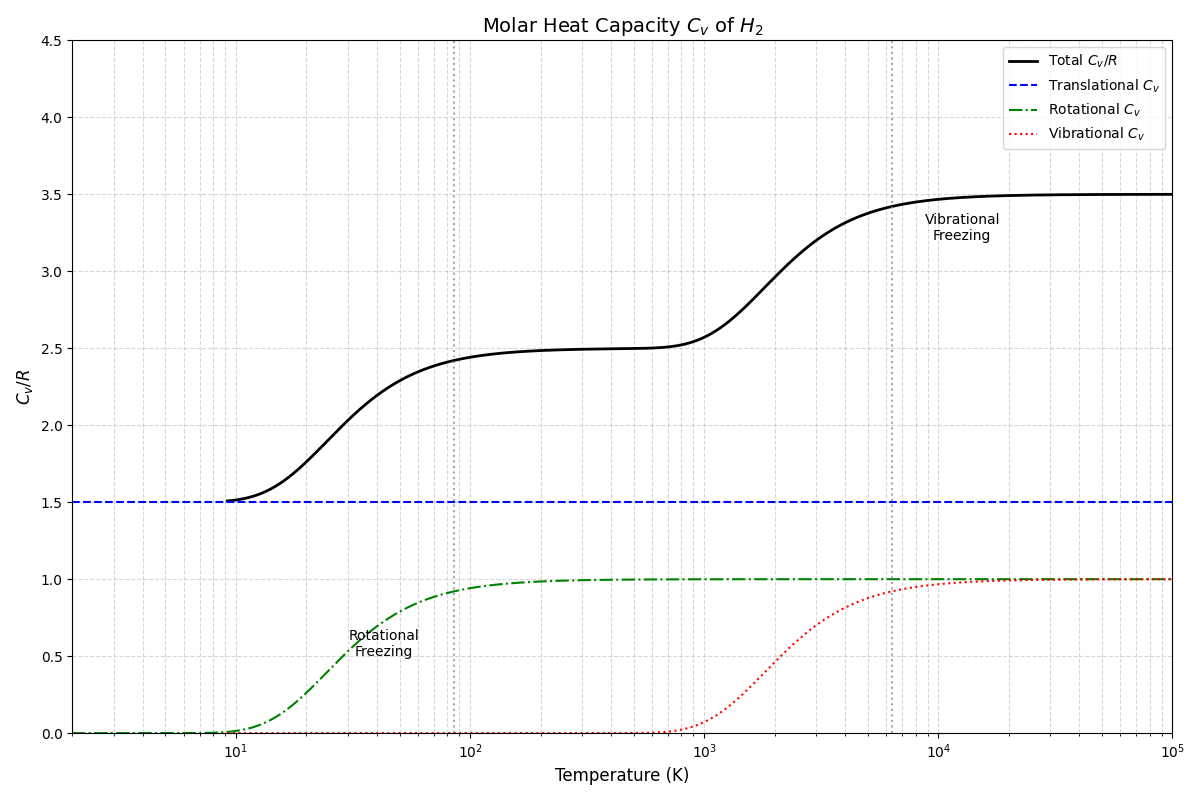
\includegraphics[width=0.7\textwidth]{H2D.png}
\end{center}

\begin{center}
    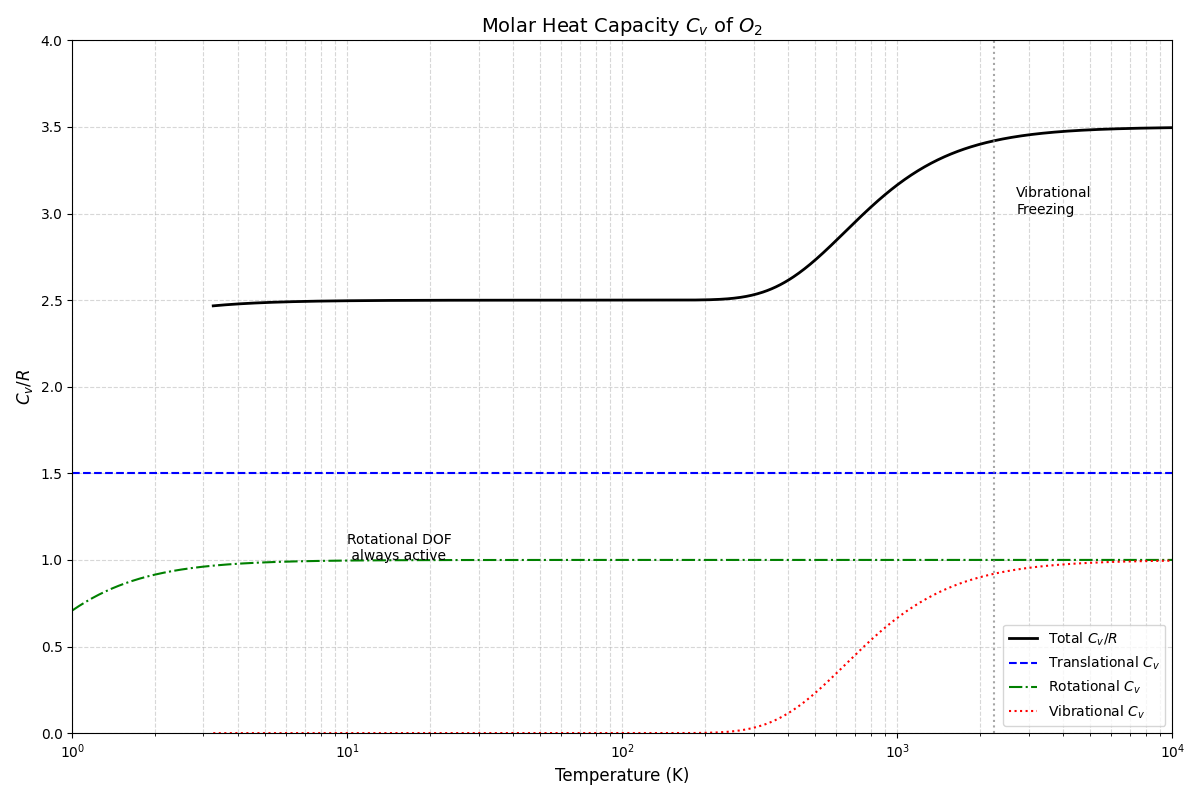
\includegraphics[width=0.7\textwidth]{O2D.png}
\end{center}

\begin{center}
    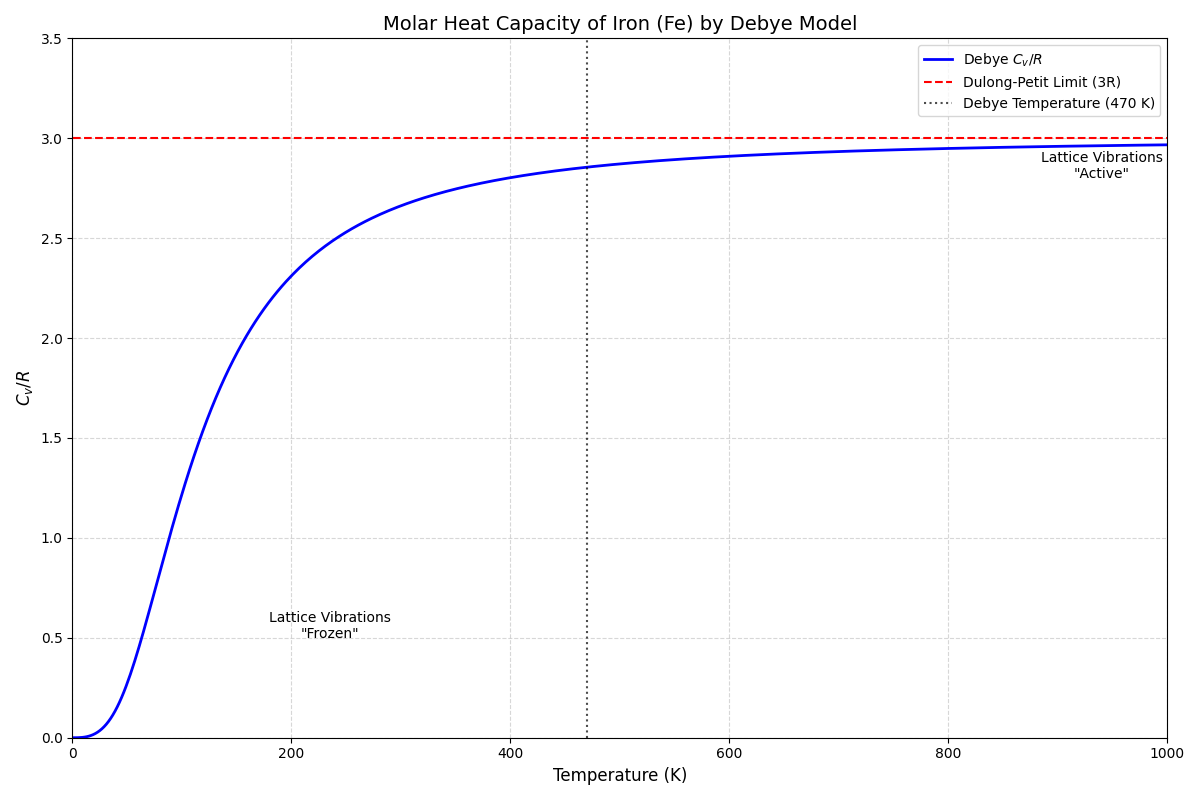
\includegraphics[width=0.7\textwidth]{FeDD.png}
\end{center}

\end{document}